\documentclass[11pt,a4paper,oneside]{report}
%\documentclass[11pt,a4paper,twoside,openright]{report}  % Duplex
\input{git_data}
% thanks to http://tex.stackexchange.com/a/47579/71109
\usepackage{ifxetex}
\usepackage{ifluatex}
\newif\ifxetexorluatex % a new conditional starts as false
\ifnum 0\ifxetex 1\fi\ifluatex 1\fi>0
   \xetexorluatextrue
\fi

\ifxetexorluatex
  \usepackage{fontspec}
  \usepackage[T1]{fontenc}
  \usepackage[utf8]{inputenc}
\else
  \usepackage[T1]{fontenc}
  \usepackage[utf8]{inputenc}
  \usepackage[lighttt]{lmodern}
  \ttfamily\DeclareFontShape{T1}{lmtt}{m}{it}{<->sub*lmtt/m/sl}{}
\fi

\usepackage[english,magyar]{babel} % Alapértelmezés szerint utoljára definiált nyelv lesz aktív, de később külön beállítjuk az aktív nyelvet.

\usepackage{emptypage} % omit page number on empty pages

%\usepackage{cmap}
\usepackage{amsfonts,amsmath,amssymb} % Mathematical symbols.
%\usepackage[ruled,boxed,resetcount,linesnumbered]{algorithm2e} % For pseudocodes. % beware: this is not compatible with LuaLaTeX, see http://tex.stackexchange.com/questions/34814/lualatex-and-algorithm2e
\usepackage{booktabs} % For publication quality tables for LaTeX
\usepackage{graphicx}

%\usepackage{fancyhdr}
%\usepackage{lastpage}

\usepackage{geometry}
%\usepackage{sectsty}
\usepackage{setspace} % For setting line spacing

\usepackage[unicode]{hyperref} % For hyperlinks in the generated document.
\usepackage{xcolor}
%\usepackage{listings} % For source code snippets.

\usepackage[outputdir=\outdir]{minted}

\usepackage[amsmath,thmmarks]{ntheorem} % Theorem-like environments.

\usepackage[hang]{caption}

\singlespacing

\newcommand{\selecthungarian}{
	\selectlanguage{magyar}
	\setlength{\parindent}{2em}
	\setlength{\parskip}{0em}
	\frenchspacing
}

\newcommand{\selectenglish}{
	\selectlanguage{english}
	\setlength{\parindent}{0em}
	\setlength{\parskip}{0.5em}
	\nonfrenchspacing
	\renewcommand{\figureautorefname}{Figure}
	\renewcommand{\tableautorefname}{Table}
	\renewcommand{\partautorefname}{Part}
	\renewcommand{\chapterautorefname}{Chapter}
	\renewcommand{\sectionautorefname}{Section}
	\renewcommand{\subsectionautorefname}{Section}
	\renewcommand{\subsubsectionautorefname}{Section}
}

\usepackage[numbers]{natbib}
\usepackage{xspace}

\usepackage{markdown}
\usepackage[show]{ed}
\usepackage{fancyhdr}

%TODO Set the main variables
\newcommand{\vikszerzoVezeteknev}{dpeter99 }
\newcommand{\vikszerzoKeresztnev}{}

\newcommand{\vikkonzulensAMegszolitas}{dr.~}
\newcommand{\vikkonzulensAVezeteknev}{-- }
\newcommand{\vikkonzulensAKeresztnev}{--}

\newcommand{\vikkonzulensBMegszolitas}{}
\newcommand{\vikkonzulensBVezeteknev}{}
\newcommand{\vikkonzulensBKeresztnev}{}

\newcommand{\vikkonzulensCMegszolitas}{}
\newcommand{\vikkonzulensCVezeteknev}{}
\newcommand{\vikkonzulensCKeresztnev}{}

\newcommand{\vikcim}{Shadow game engine} % Cím
\newcommand{\viktanszek}{\bmemit} % Tanszék
\newcommand{\vikdoktipus}{\bsc} % Dokumentum típusa (\bsc vagy \msc)
\newcommand{\vikmunkatipusat}{szakdolgozatot} % a "hallgató nyilatkozat" részhez: szakdolgozatot vagy diplomatervet

%--------------------------------------------------------------------------------------
% TDK-specifikus változók
%--------------------------------------------------------------------------------------
\newcommand{\tdkszerzoB}{Második Szerző} % Második szerző neve; hagyd üresen, ha egyedül írtad a TDK-t.
\newcommand{\tdkev}{2014} % A dolgozat írásának éve (pl. "2014") (Ez OTDK-nál eltérhet az aktuális évtől.)

% További adatok az OTDK címlaphoz (BME-s TDK-hoz nem kell kitölteni)
\newcommand{\tdkevfolyamA}{IV} % Első szerző évfolyama, római számmal (pl. IV).
\newcommand{\tdkevfolyamB}{III} % Második szerző évfolyama, római számmal (pl. III).
\newcommand{\tdkkonzulensbeosztasA}{egyetemi tanár} % Első konzulens beosztása (pl. egyetemi docens)
\newcommand{\tdkkonzulensbeosztasB}{doktorandusz} % Második konzulens beosztása (pl. egyetemi docens)

\newcommand{\szerzoMeta}{\vikszerzoVezeteknev \vikszerzoKeresztnev} % egy szerző esetén
%\newcommand{\szerzoMeta}{\vikszerzoVezeteknev{} \vikszerzoKeresztnev, \tdkszerzoB} % két szerző esetén

%TODO Language configuration -- choose one
% Beállítások magyar nyelvű dolgozathoz
%\input{includes/thesis-hu}
% Settings for English documents
%--------------------------------------------------------------------------------------
% Elnevezések
%--------------------------------------------------------------------------------------
\newcommand{\bme}{Budapest University of Technology and Economics}
\newcommand{\vik}{Faculty of Electrical Engineering and Informatics}

\newcommand{\bmemit}{Department of Measurement and Information Systems}

\newcommand{\keszitette}{Author}
\newcommand{\konzulens}{Advisor}

\newcommand{\bsc}{Bachelor's Thesis}
\newcommand{\msc}{Master's Thesis}
\newcommand{\tdk}{Scientific Students' Association Report}
\newcommand{\bsconlab}{BSc Project Laboratory}
\newcommand{\msconlabi}{MSc Project Laboratory 1}
\newcommand{\msconlabii}{MSc Project Laboratory 2}

\newcommand{\pelda}{Example}
\newcommand{\definicio}{Definition}
\newcommand{\tetel}{Theorem}

\newcommand{\bevezetes}{Introduction}
\newcommand{\koszonetnyilvanitas}{Acknowledgements}
\newcommand{\fuggelek}{Appendix}

% Optional custom titles
%\addto\captionsenglish{%
%\renewcommand*{\listfigurename}{Your list of figures title}
%\renewcommand*{\listtablename}{Your list of tables title}
%\renewcommand*{\bibname}{Your bibliography title}
%}

\newcommand{\szerzo}{\vikszerzoVezeteknev \vikszerzoKeresztnev{}}
\newcommand{\vikkonzulensA}{\vikkonzulensAMegszolitas \vikkonzulensAVezeteknev \vikkonzulensAKeresztnev{}}
\newcommand{\vikkonzulensB}{\vikkonzulensBMegszolitas \vikkonzulensBVezeteknev \vikkonzulensBKeresztnev{}}
\newcommand{\vikkonzulensC}{\vikkonzulensCMegszolitas \vikkonzulensCVezeteknev \vikkonzulensCKeresztnev{}}

\newcommand{\selectthesislanguage}{\selectenglish}

\bibliographystyle{plainnat}

\newcommand{\ie}{i.e.\@\xspace}
\newcommand{\Ie}{I.e.\@\xspace}
\newcommand{\eg}{e.g.\@\xspace}
\newcommand{\Eg}{E.g.\@\xspace}
\newcommand{\etal}{et al.\@\xspace}
\newcommand{\etc}{etc.\@\xspace}
\newcommand{\vs}{vs.\@\xspace}
\newcommand{\viz}{viz.\@\xspace} % videlicet
\newcommand{\cf}{cf.\@\xspace} % confer
\newcommand{\Cf}{Cf.\@\xspace}
\newcommand{\wrt}{w.r.t.\@\xspace} % with respect to
\newcommand{\approximately}{approx.\@\xspace}

\newcommand{\appendixnumber}{1}  % a fofejezet-szamlalo az angol ABC 1. betuje (A) lesz


%--------------------------------------------------------------------------------------
% Page layout setup
%--------------------------------------------------------------------------------------
% we need to redefine the pagestyle plain
% another possibility is to use the body of this command without \fancypagestyle
% and use \pagestyle{fancy} but in that case the special pages
% (like the ToC, the References, and the Chapter pages)remain in plane style

\pagestyle{plain}
\geometry{inner=35mm, outer=25mm, top=28mm, bottom=25mm}

\setcounter{tocdepth}{3}
%\sectionfont{\large\upshape\bfseries}
\setcounter{secnumdepth}{3}

\sloppy % Margón túllógó sorok tiltása.
\widowpenalty=10000 \clubpenalty=10000 %A fattyú- és árvasorok elkerülése
\def\hyph{-\penalty0\hskip0pt\relax} % Kötőjeles szavak elválasztásának engedélyezése


%--------------------------------------------------------------------------------------
% Setup hyperref package
%--------------------------------------------------------------------------------------
\hypersetup{
    % bookmarks=true,            % show bookmarks bar?
    unicode=true,              % non-Latin characters in Acrobat's bookmarks
    pdftitle={\vikcim},        % title
    pdfauthor={\szerzoMeta},    % author
    pdfsubject={\vikdoktipus}, % subject of the document
    pdfcreator={\szerzoMeta},   % creator of the document
    pdfproducer={},    % producer of the document
    pdfkeywords={},    % list of keywords (separate then by comma)
    pdfnewwindow=true,         % links in new window
    colorlinks=true,           % false: boxed links; true: colored links
    linkcolor=black,           % color of internal links
    citecolor=black,           % color of links to bibliography
    filecolor=black,           % color of file links
    urlcolor=black             % color of external links
}
\providecommand*{\listingautorefname}{Listing}

%--------------------------------------------------------------------------------------
% Set up listings
%--------------------------------------------------------------------------------------
%\definecolor{lightgray}{rgb}{0.95,0.95,0.95}
%\lstset{
%	basicstyle=\scriptsize\ttfamily, % print whole listing small
%	keywordstyle=\color{black}\bfseries, % bold black keywords
%	identifierstyle=, % nothing happens
%	% default behavior: comments in italic, to change use
%	% commentstyle=\color{green}, % for e.g. green comments
%	stringstyle=\scriptsize,
%	showstringspaces=false, % no special string spaces
%	aboveskip=3pt,
%	belowskip=3pt,
%	backgroundcolor=\color{lightgray},
%	columns=flexible,
%	keepspaces=true,
%	escapeinside={(*@}{@*)},
%	captionpos=b,
%	breaklines=true,
%	frame=single,
%	float=!ht,
%	tabsize=2,
%	literate=*
%		{á}{{\'a}}1	{é}{{\'e}}1	{í}{{\'i}}1	{ó}{{\'o}}1	{ö}{{\"o}}1	{ő}{{\H{o}}}1	{ú}{{\'u}}1	{ü}{{\"u}}1	{ű}{{\H{u}}}1
%		{Á}{{\'A}}1	{É}{{\'E}}1	{Í}{{\'I}}1	{Ó}{{\'O}}1	{Ö}{{\"O}}1	{Ő}{{\H{O}}}1	{Ú}{{\'U}}1	{Ü}{{\"U}}1	{Ű}{{\H{U}}}1
%}

%\setmonofont[
%Path=./common/fonts/JetbrainsMono/,
%Scale=0.85,
%Extension=.ttf,
%UprightFont=*-Regular,
%BoldFont=*-Bold,
%ItalicFont=*-Italic,
%BoldItalicFont=*-BoldItalic
%]{JetBrainsMono}

%\newfontfamily\JBMono{JetBrainsMono}[NFSSFamily=JetBrainsMono]
%\setminted[matlab]{fontfamily=JetBrainsMono}


%--------------------------------------------------------------------------------------
% Set up theorem-like environments
%--------------------------------------------------------------------------------------
% Using ntheorem package -- see http://www.math.washington.edu/tex-archive/macros/latex/contrib/ntheorem/ntheorem.pdf

\theoremstyle{plain}
\theoremseparator{.}
\newtheorem{example}{\pelda}

\theoremseparator{.}
%\theoremprework{\bigskip\hrule\medskip}
%\theorempostwork{\hrule\bigskip}
\theorembodyfont{\upshape}
\theoremsymbol{{\large \ensuremath{\centerdot}}}
\newtheorem{definition}{\definicio}

\theoremseparator{.}
%\theoremprework{\bigskip\hrule\medskip}
%\theorempostwork{\hrule\bigskip}
\newtheorem{theorem}{\tetel}


%--------------------------------------------------------------------------------------
% Some new commands and declarations
%--------------------------------------------------------------------------------------
\newcommand{\code}[1]{{\upshape\ttfamily\scriptsize\indent #1}}
\newcommand{\doi}[1]{DOI: \href{http://dx.doi.org/\detokenize{#1}}{\raggedright{\texttt{\detokenize{#1}}}}} % A hivatkozások közt így könnyebb DOI-t megadni.

\DeclareMathOperator*{\argmax}{arg\,max}
%\DeclareMathOperator*[1]{\floor}{arg\,max}
\DeclareMathOperator{\sign}{sgn}
\DeclareMathOperator{\rot}{rot}


%--------------------------------------------------------------------------------------
% Setup captions
%--------------------------------------------------------------------------------------
\captionsetup[figure]{aboveskip=10pt}

\renewcommand{\captionlabelfont}{\bf}
%\renewcommand{\captionfont}{\footnotesize\it}

%--------------------------------------------------------------------------------------
% Hyphenation exceptions
%--------------------------------------------------------------------------------------
\hyphenation{Shakes-peare Mar-seilles ár-víz-tű-rő tü-kör-fú-ró-gép}


\author{\vikszerzo}
\title{\viktitle}


\newfontface\lserif{Liberation Serif}
\newcommand{\Csh}{C{\lserif\#}}
\newcommand{\Cpp}{C\nolinebreak\hspace{-.05em}\raisebox{.4ex}{\tiny\bf +}\nolinebreak\hspace{-.10em}\raisebox{.4ex}{\tiny\bf +}}

%--------------------------------------------------------------------------------------
% Table of contents and the main text
%--------------------------------------------------------------------------------------
\begin{document}

    \pagenumbering{gobble}

    \selectthesislanguage

%TODO Titlepage -- choose one from below
%~~~~~~~~~~~~~~~~~~~~~~~~~~~~~~~~~~~~~~~~~~~~~~~~~~~~~~~~~~~~~~~~~~~~~~~~~~~~~~~~~~~~~~
    \hypersetup{pageanchor=false}
%--------------------------------------------------------------------------------------
%	The title page
%--------------------------------------------------------------------------------------
\begin{titlepage}
    \begin{center}
        
\includegraphics[width=60mm,keepaspectratio]{common/figures/bme_logo.pdf}\\
        \vspace{0.3cm}
        \textbf{\bme}\\
        \textmd{\vik}\\
        \textmd{\viktanszek}\\[5cm]

        \vspace{0.4cm}
        {\huge \bfseries \vikcim}\\[0.8cm]
        \vspace{0.5cm}
        \textsc{\Large \vikdoktipus}\\[4cm]

        {
            \renewcommand{\arraystretch}{0.85}
            \begin{tabular}{cc}
                \makebox[7cm]{\emph{\keszitette}} & \makebox[7cm]{\emph{\konzulens}} \\ \noalign{\smallskip}
                \makebox[7cm]{\szerzo}            & \makebox[7cm]{\vikkonzulensA}    \\
                & \makebox[7cm]{\vikkonzulensB}    \\
                & \makebox[7cm]{\vikkonzulensC}    \\
            \end{tabular}
        }

        \vfill
        %{\large \today \linebreak \gitcommit - \gitbranch}

    \end{center}
\end{titlepage}
\hypersetup{pageanchor=false}

           % Szakdolgozat/Diplomaterv címlap
%\include{include/titlepage-tdk}	% TDK címlap
%\include{include/titlepage-otdk}   % OTDK címlap


% Table of Contents
%~~~~~~~~~~~~~~~~~~~~~~~~~~~~~~~~~~~~~~~~~~~~~~~~~~~~~~~~~~~~~~~~~~~~~~~~~~~~~~~~~~~~~~
    \tableofcontents\cleardoublepage


% Declaration and Abstract
%~~~~~~~~~~~~~~~~~~~~~~~~~~~~~~~~~~~~~~~~~~~~~~~~~~~~~~~~~~~~~~~~~~~~~~~~~~~~~~~~~~~~~~
    \selectlanguage{magyar}
\pagenumbering{gobble}
%--------------------------------------------------------------------------------------
% Nyilatkozat
%--------------------------------------------------------------------------------------
\begin{center}
\large
\textbf{HALLGATÓI NYILATKOZAT}\\
\end{center}

Alulírott \emph{\vikszerzoVezeteknev{} \vikszerzoKeresztnev}, szigorló hallgató kijelentem, hogy ezt a \vikmunkatipusat{} meg nem engedett segítség nélkül, saját magam készítettem, csak a megadott forrásokat (szakirodalom, eszközök stb.) használtam fel. Minden olyan részt, melyet szó szerint, vagy azonos értelemben, de átfogalmazva más forrásból átvettem, egyértelműen, a forrás megadásával megjelöltem.

Hozzájárulok, hogy a jelen munkám alapadatait (szerző(k), cím, angol és magyar nyelvű tartalmi kivonat, készítés éve, konzulens(ek) neve) a BME VIK nyilvánosan hozzáférhető elektronikus formában, a munka teljes szövegét pedig az egyetem belső hálózatán keresztül (vagy autentikált felhasználók számára) közzétegye. Kijelentem, hogy a benyújtott munka és annak elektronikus verziója megegyezik. Dékáni engedéllyel titkosított diplomatervek esetén a dolgozat szövege csak 3 év eltelte után válik hozzáférhetővé.

\begin{flushleft}
\vspace*{1cm}
Budapest, \today
\end{flushleft}

\begin{flushright}
 \vspace*{1cm}
 \makebox[7cm]{\rule{6cm}{.4pt}}\\
 \makebox[7cm]{\emph{\vikszerzoVezeteknev{} \vikszerzoKeresztnev}}\\
 \makebox[7cm]{hallgató}
\end{flushright}
\thispagestyle{empty}

\vfill
\cleardoublepage

\selectthesislanguage
 %TODO Hallgatói nyilatkozat -- TDK és OTDK esetén törlendő!
    %\include{content/abstract}    %TODO Összefoglaló -- TDK és OTDK esetén nem kötelező


% The main part of the thesis
%~~~~~~~~~~~~~~~~~~~~~~~~~~~~~~~~~~~~~~~~~~~~~~~~~~~~~~~~~~~~~~~~~~~~~~~~~~~~~~~~~~~~~~

    \pagestyle{fancy}
    \fancyhf{}
    \renewcommand{\headrulewidth}{0pt}
    \fancyfoot[C]{\thepage}
    %\fancyfoot[R]{\\ \today \, \gitcommitshort \, \gitbranch}

    % Redefine the plain page style
    \fancypagestyle{plain}{
        \fancyhf{}
        \fancyfoot[C]{\thepage}
    %\fancyfoot[R]{\\ \today \, \gitcommitshort \, \gitbranch}
    }

    \pagenumbering{roman}
\setcounter{page}{1}

\selecthungarian

%----------------------------------------------------------------------------
% Abstract in Hungarian
%----------------------------------------------------------------------------
\chapter*{Kivonat}\addcontentsline{toc}{chapter}{Kivonat}

A szakdolgozat projektem célja egy játék motor készítése, ami a jelenleg is elérhetőkéhez hasonló képességekkel bír.
Mivel ez egy rendkívülien nagy feladat, amit nem lehet a szakdolgozat ideje alatt befejezni, ezért a projekt jó megalapozására fókuszáltam.
Ez azt jelenti, hogy több időt fektettem a megfelelő eszközök kiválasztásába, mint amennyit más esetekben fordítanék erre.
Ilyen volt például a projektben, a kód fordítására használt eszközök megválasztása.
A szakdolgozattal véleményem szerint egy jó alapot tudtam adni a projektemnek, aminek a fejlesztését a jövőben is szeretném folytatni.
Megvalósított részek:

\begin{itemize}
    \item A fordítási környezet megtervezése
    \item Dinamikus, kód betöltés a motor modulokhoz
    \item Kezdeti entitás rendszer
    \item Kód reflexió megvalósítása \Cpp-ban
\end{itemize}

Egy ismerősöm felajánlotta, hogy segít a motor grafikus részének megírásában, azonban a szakdolgozatban csak a saját kódomat fogom bemutatni.
A projekt GitHub-on található és MIT licenszelésű.
A források elérhetőek a következő linken: \url{https://github.com/dpeter99/umbra/tree/thesis} a \verb|thesis| branch-en.


\vfill
\selectenglish


%----------------------------------------------------------------------------
% Abstract in English
%----------------------------------------------------------------------------
\chapter*{Abstract}\addcontentsline{toc}{chapter}{Abstract}

This project's goal is to create a game engine similar in design to currently available big commercial engines.
As this is a large proposal that far exceeds the limits and practicality of a thesis project, I was focusing on giving the project a good foundation.
This means that, I have spent considerable amount of time on investigating solutions to issues other projects would not care about like build systems and project organization.
By the end, I think I have created a solid foundation including the core systems for the engine that I plan to use, and continue working on in the coming years.
Finished parts:

\begin{itemize}
    \item Choosing a build system that is usable with large projects
    \item Dynamic DLL loading of engine modules
    \item Basic Entity system
    \item Reflection system for runtime code metadata
\end{itemize}


A friend of mine has offered to write the renderer for the engine, however, I will be only presenting the parts that are entirely my own.

The project is hosted on GitHub and is MIT licensed.

The source code is available at \url{https://github.com/dpeter99/umbra/tree/thesis} under the \verb|thesis| branch.


\vfill
\selectthesislanguage

\newcounter{romanPage}
\setcounter{romanPage}{\value{page}}
\stepcounter{romanPage}

    % The main part of the thesis
    %~~~~~~~~~~~~~~~~~~~~~~~~~~~~~~~~~~~~~~~~~~~~~~~~~~~~~~~~~~~~~~~~~~~~~~~~~~~~~~~~~~~~~~
    \pagenumbering{arabic}

    \chapter{Abstract}
% Short summary
This projects goal is to create a game engine, similar in design to currently available big commercial engines.
As this is a large undertaking that far exceeds the limits and practicality of a thesis project, I will be focusing on giving the project a good foundation. This means considerable amount of time will be spent investigating solutions to issues other projects would not care about. By the end I hope to have a solid foundation and core systems for the engine that I plan to use and extend in the coming years.
Planned parts:

\begin{itemize}
    \item CI/CD pipelines
    \item Choosing a build system that is usable with large projects
    \item Dynamic DLL loading of engine modules
    \item Basic Entity system
    \item Reflection system for runtime code metadata
\end{itemize}

The project is a collaboration between me and a friend of mine, she will be writing the renderer and donating some other bits of code. The parts that I will be presenting are entirely my own.

The project is hosted on GitHub and is MIT licensed.


\chapter{Intro}

The most well known computer games are usually mobile games like Candy Crush \cite{candy-crush} or bigger budget console games like The Last of Us \footnote{This game series recently even got a really successful TV adaptation by HBO}\cite{last-of-us}. But there are many different types of video games, that present vastly different experiences. For example, there are games that play entirely in a text based window and focus on the story, while others don't have any story and are based on multiple players interacting. But all of these are pieces of software that need a lot of different disciplines to work together in order to create them. At the bare minimum, one needs to be a good software engineer to create the code for the game and also be able to design a good and engaging game. But when it comes to large production games, so-called "AAA" or "triple A" games, the number of necessary tasks increases. For these games on top of the programming and game design new tasks come in like story writing, 3D modelling, environment design, level design, music, and countless others. For these games, there is an expectation to excel in every category or even push the bounds of what is possible.

Because video games as so complex, there is a need to share some of the code between projects, as starting from scratch for each is impractical. This is possible because many of the functionality needed to create a game is the same for every game. For example, almost all games need a way to show 3D models on the display, and they need to process input from the player, regardless of what the actual gameplay is. These more abstract, not game specific functionalities, can be shared between projects.

These sharable functionalities are what form many of the game development code libraries. These are not runnable code by themselves and are only for the programmers to help and accelerate creating a game. A great example of such a code library is \verb|raylib| \cite{raylib} which can provide many of the important functionality for the developer, such as graphics, 3D model loading and textures, and even audio playback. Game engines are even more complex, and are responsible for running the actual game application. In most cases, they include editors and tools to create the assets that are going to be used in the game. This usually includes a world editor to create the 2D or 3D environment the player can explore.

There are many game engines, but it is important to highlight that not all of them are publicly available. Most of the video game studios that create their own game engines, so called "in-house" engines, usually never make them available for public usage. On the other hand, there are public engines that everybody can use to create their own games, some of these are completely free, while others require some payment for the usage. As the in house engines are treated as trade secrets people rarely share details about them, the most we can learn is from conference talks.

I have been using Unity - one of the most popular game engines - since 2015, and have been fascinated by how games work way before that. Using Unity, I have created many basic projects and prototypes. These were usually too ambitious projects for me alone to achieve them, but gave the chance to explore and try out many aspects of the engine. Using a popular commercial engine also allowed me to better understand what a game creator expects from an engine and what are the most critical things when creating a game. As my coding skills expanded and my goals became more realistic, I have started finding more and more pain points in Unity. This has become extremely evident in the last major project I did in Unity, which was for the "Project Laboratory" course. In that project, I have implemented a complex extension that helped to create gameplay logic. \cite{szájberpunk-logic-system}. During this last project, I have found myself "fighting" with unity more than actually enjoying the development.

I have experimented with writing my own game engine multiple time with many different technologies and ways to approach the problem. The first substantial try was back in the last year of high school with the project codenamed: \verb|Cryogenic-engine| where I tried to use C\# and the Vulkan graphics API. With this project I ran into many classical mistakes, and it showed me how large and complex a game engine can be. For example, the Vulkan API that I have chosen for drawing to the screen is not beginner-friendly and is really hard to understand. On the other hand, it is a powerful way of interacting with the GPU. The start of university caused me to put this project on hold and later abandon it fully.

During my University years, I have worked on 2 other game engines. The first one was \verb|relic engine| which was written in the first semester for the "Basics of Programming 1" (C coding course). This was a simple 2D game engine the was able to load in tile based maps and allow for basic gameplay. I wrote this in a single semester while learning the C programming language as well. After this, I have started working on the predecessor of this project, nicknamed \verb|Old Shadow Engine|. This was at first going to be a simple rewrite of \verb|relic Engine| but I kept extending it with new feature ideas before finishing the base \footnote{When the planned features balloon up like this it is called feature creep in the programming industry}.

Based on my frustrations with existing engines and my prior experience writing creating basic ones, the idea of making one for my thesis project came naturally. The initial push and encouragement for the project came from one of my online friend, who agreed to even help with writing the rendering code for the engine. My basic idea was to start from scratch and re-do what I have done with the old Shadow Engine, but this time do it right. This is why I kept the name for the project, but as this time hopefully multiple people are going to be working on this, I have created a GitHub group for it and a fresh new code repository. 

Choosing the right technologies for such a project is really important, as some changes are practicality impossible to change later. The most important choice is the programming language, as this influences all other choices I have to make. I chose to use C++ as I already have some experience with it - mainly with the old Shadow Engine project -, and this is the industry standard for making games. I have also considered other similar languages like Rust, but I have decided against it in order to allow as many people to contribute as possible. The next big decision was to decide on a build system that will help in compiling the potentially enormous codebase. This was a longer and more complex decision, and I will be detailing it later in \autoref{}.


    \chapter{Existing solutions}\label{chapter:research}

There are many existing game engines, and I think it is important for me to examine where they succeed and where they fail so I can learn from them. Sadly, as I have mentioned, there aren't many engines that we can use for free, and there are even fewer engines where we can see the source code as well. In this section I will be presenting a few of the existing engines and what I think their strong points and mistakes are.
As I have the most experience with Unity I will be exploring it in more detail than the others.


\section{Unity}

The Unity game engine\cite{unity}, developed by Unity Technologies, is an extensive platform known for creating many types of interactive content, with a primary emphasis on video games, but it is also used in simulations or architectural visualization. This engine allows the creation of 2D, 3D, and virtual reality (VR) games for almost every platform, such as Windows, macOS, Linux, Mobile, and consoles. Unity rose in popularity due to its cross-platform capabilities, easy to use environment, and the supportive community that formed around it. It uses \Csh as the primary scripting language, which is known for its versatility and efficiency, this also made it popular among developers. Additionally, its intuitive design and the availability of extensive learning resources have made Unity highly accessible, propelling its popularity.

In Unity, the game's world - called Scene - is built from Game Objects, which can represent anything that is necessary for the gameplay. Most commonly these include the player and the environment they are in, but can also be more abstract things like managers for different game systems. To give these Game Objects logic, the user needs to add Components to them. One of the most common components are Mesh and Mesh Renderer which make the Game Object show up in the game world. The engine has many other built in components that can add physics, rendering, sound and many other capabilities to the objects. If the built-in set of components are not enough, than the user can create custom components by writing \Csh scripts that extend the \verb|MonoBehaviour| base class. The game objects can be attached to each other called "parenting", this causes them to move together with the parent object. This is commonly used to make a camera or a clothes follow the player.

These scenes are authored inside the editor using the Scene view, Hierarchy, and Inspector sections. In the scene view, we have a bird's eye view of the environment we are creating, while the Hierarchy and Inspector views provide a more abstract way of editing the scene. The Hierarchy (\autoref{fig:unity-hierarchy}) shows a list of all the Game Objects that are present in the scene, because these can have parent-children relations this view forms a tree.

Inspector (\autoref{fig:unity-inspector}) is a view that shows the properties of the currently selected object. This view is used to edit the properties of the Game Object, the Components attached to it, and to add new components to it.

Despite Unity's popularity in the independent developer community (called "indie" developers) and huge success in creating diverse games, it is not without shortcomings. One of the most glaring issues I have encountered have been with the sporadic updates. Unity seams to be focused on chasing the newest and most cutting edge technologies, but this often results in a neglect of existing bugs and stability issues. As a long time user, it feels like the engine has become more and more cluttered with new half finished features, and even more bugs. Many of the new features announced years ago are still in development, and many others have been silently discontinued.

Because of this constant chase of the new technologies, there are many areas where multiple competing solutions exist for a single problem. The most infamous example is the networking libraries, where there are multiple solutions. These make the developer's choice for what system to use harder, as older solution might be unsupported in the next engine version, but the replacement is not yet ready in the current version. This makes even starting a new project really hard and require a lot of unnecessary decisions.

\begin{figure}[h]
    \centering
    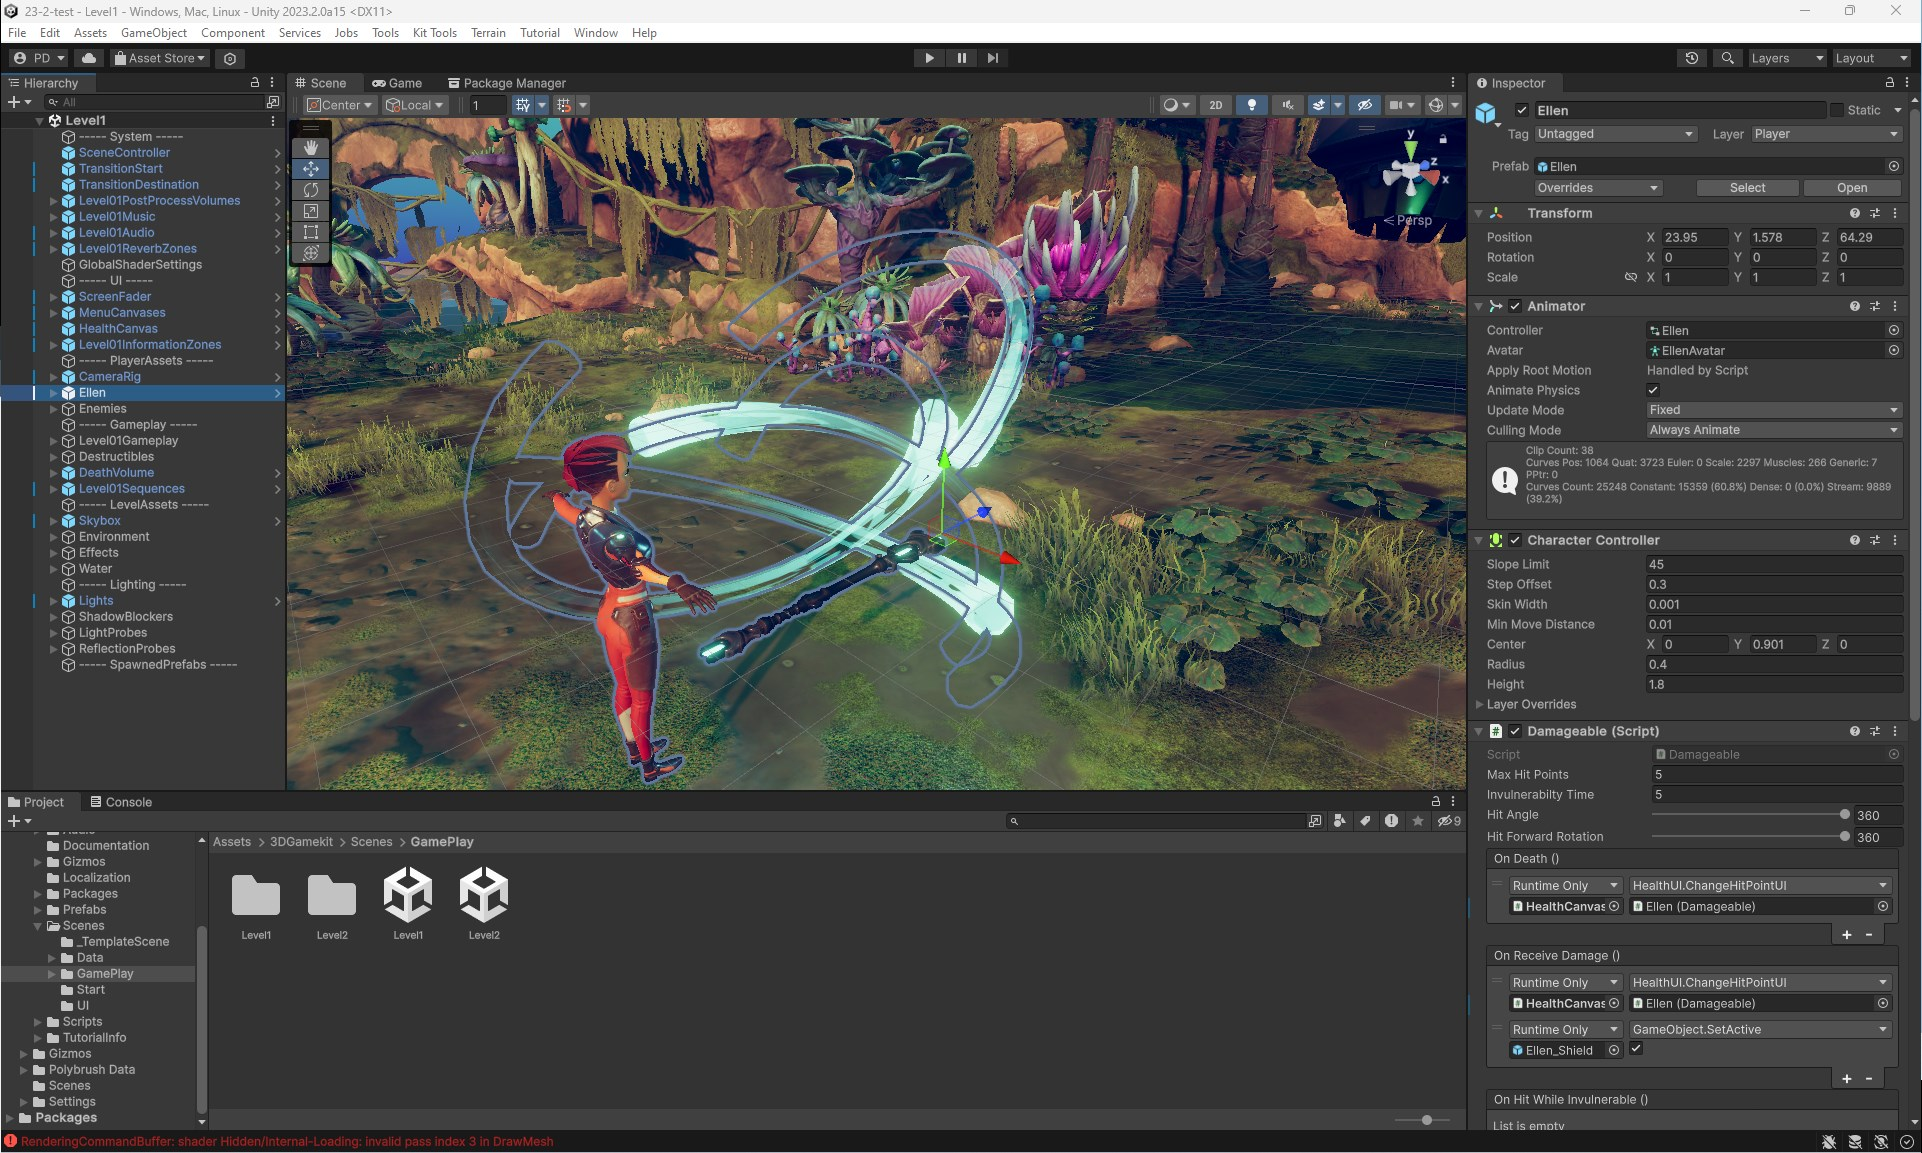
\includegraphics[width=\textwidth]{content/Research/Unity-Editor-2.jpg}
    \caption{Screenshot of the Unity engine's unified editor.}
    \label{fig:unity-editor}
\end{figure}


\section{Unreal Engine 5}

Unreal Engine (UE), developed by Epic Games, has a rich and long history that has significantly influenced the landscape of modern gaming. The inception of Unreal Engine dates back to 1998, when the first-person shooter game 'Unreal'\cite{unreal-game} was released. Since then, it has undergone several mayor transformations, resulting in its latest iteration Unreal Engine 5 (UE5). Throughout the years, the engine has consistently pushed the boundaries of what's possible in game development, from pioneering high-fidelity graphics to realizing expansive virtual worlds.

Unreal Engine 5, boasts a tremendous leap forward in visual fidelity, by using groundbreaking technologies such as Nanite and Lumen.
Nanite is a system that essentially eliminates the limitations of polygon count and draw call overheads in 3D environment modelling. It achieves this by using so-called "virtual polygons", allowing for much greater model detail to be used without major performance hit. This system can replace the traditional Level Of Detail (LOD)\footnote{A system where separate models are created for when the given object is further away.} approach, allowing for much faster development time.
Lumen, on the other hand, is a fully dynamic global illumination solution that can immediately react to scene and light changes, producing more lifelike environments. It is important to highlight that while these technologies can produce stunning visuals, they are slower than traditional approaches and not suitable for every game, or platform.


\begin{figure}[h]
    \centering
    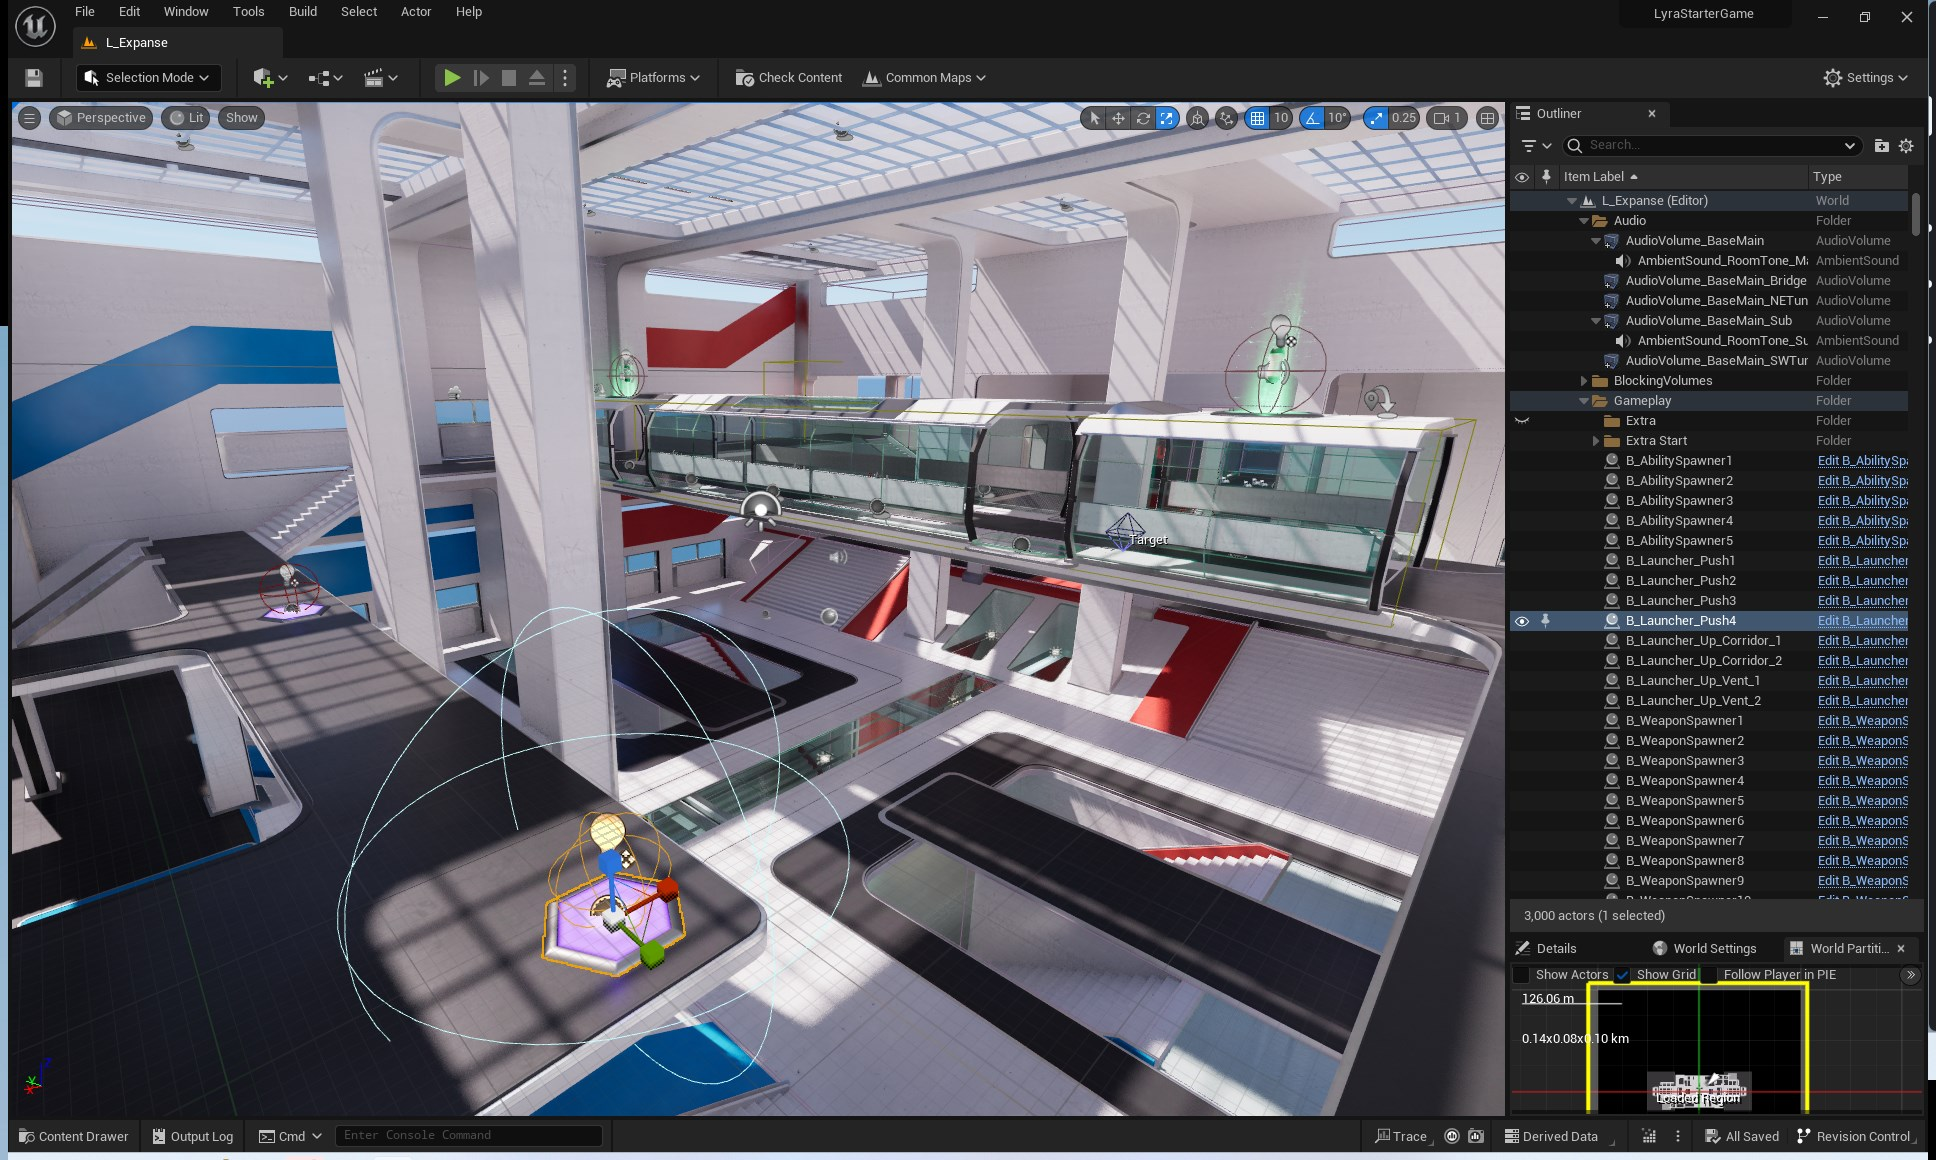
\includegraphics[width=0.8\textwidth]{content/Research/UE5-editor}
    \caption{Screenshot of the Unreal Engine 5 editor.}
    \label{fig:ue5-editor}
\end{figure}

\subsection{Actors and the Outliner}

In UE 5, the fundamental building blocks of a game world are called Actors. An Actor is essentially any object that can be placed into the game world, and they can represent characters, scenery, and even complex gameplay elements. There are many built in Actors that do common functionality, for example common game objects such as characters, cameras, lights, and physics objects.

The list of the Actors present in the game world is shown in the Outliner witch is a tool within UE5 editor that provides a hierarchical view of all the Actors present in a level (\autoref{fig:ue5-outliner}).

Components are the building blocks of Actors, and they can be thought of as the individual features that make up an Actor. For example, a character Actor might have a Mesh Component, a Camera Component, and a Character Movement Component. Components can form a parent-child relationship inside an Actor. This allows for the creation of complex Actors. The list of components present in an Actor is shown in the Details panel (\autoref{fig:ue5-details}), this shows the hierarchy of the components and their properties.

But the user also has multiple options to create new types specific to their game. One such method is through the use of Blueprints, a visual scripting system that allows for the creation of custom Actors without the need for traditional programming. This system uses visual nodes to define the code flow, and is quite beginner-friendly. By combining pre-existing components and defining their interactions through Blueprint nodes, developers can create new Actor types that fit their game's requirements.

Another method for creating new Actor types is through \Cpp programming.
UE5 is written in \Cpp and natively only supports \Cpp based scripting, but plugins exist which allow for other languages like \Csh to be used for coding. These methods are more complex and requires a good understanding of \Cpp and the UE5 API, but it allows for more advanced functionality and performance optimizations.


    \chapter{Planning}\label{chapter:planning}

% Description of what the plan is for this game engine.


My goal for this project is to start creating a game engine that I can work on in the future, and hopefully gather many of my friends to help me as well. 
Given the complexity and scope of this endeavour, it's crucial to start with a solid foundation.
For this regard, I have looked into many of the popular game engines as outlined in \autoref{chapter:research} and tried to pick the best ideas from each. 
For a successful open source project, it is important to make contributing as easy as possible, while also planning for growth of the project. Keeping this in mind was really important for me while choosing technologies to use, and will be detailing more in \autoref{}

\section{Modular Design}

Both Unity and Unreal engines have a modular design to ensure flexibility, extensibility, and manageability. Modules allow for separation of concerns, making it easier for contributors to understand, modify, and test individual components of the engine without interfering with others. 
A well-structured modular design allows for parallel development of different aspects of the game. This is really important for me as this large project is a collaborative effort from the start, with my friend making the renderer.
On to of this, modular design also enables the engine to adapt to a wide range of game genres and requirements, while not bloating the core of the engine with code that is not useful for the given game. For example, a VR module can only be enabled and loaded when it is actually necessary. Modularity is therefore a critical feature of the engine I want to create.

\section{Unified Editor}

The other important take away from examining existing game engines was that while many allowed for, most of them didn't need to compile the engine and editor for the given game. On top of this, another common aspect was that modern engines had all the editor tools integrated into a single application. This made development much easier and faster to learn. These mean a lot of time can be saved while developing the actual games, but they definitely add to the complexity of the project.

To give the engine the ability to load in the game code while running and not need to compile it together with the engine, the game code needs to be a separate compilation step. The engine needs to be able to load in this separate code and also reload it when it gets recompiled. This is a more tricky problem than it would first seam, as it needs to correctly link the external code.

To create a game engine where all necessary authoring tools are built into the editor is certainly possible, but would take exponentially longer than this thesis project allows. Because of this I will be not focusing on this aspect but leaving it for future development. In the meantime, I will be using external industry standard editors to create assets for testing.

\section{Entity system}

Every game engine needs a way to represent the game world in code in some way. In Unity there are the \verb|GameObject|s, in UE they are \verb|Actor|s, while valve's Source engine calls them Entities, but they fulfil a functionally similar role in making a game. As we can see from just these examples, there isn't an industry standard way of naming these building blocks, and their implementation also differs between engines greatly.

While in Unity and Unreal the user adds Components to create functionality, in Source all entities are pre-defined, and new ones can only be added using \Cpp \footnote{There are some Source games that support easier scripting with VScript \cite{valve-vscript}}. But Unity and UE also differ in their approach where Unity only has a flat list of components, UE allows for a whole internal hierarchy of components.
    \chapter{Project Setup}\label{chap:project-setup}

In order to even start creating such a huge project I need to decide on a build system to use, and decide on many other developer tools.

Choosing Git for version management was an obvious chose for me, as it is the platform that most of the open source development efforts use. This is mainly because of it's versatility and relative ease of use. For hosting, I will be using GitHub as it has a generous free tier, that includes free cloud builds witch I'm planning on using in this project.

When it comes to structuring the project, I have decided to use a true monorepo approach, where everything relating to the project will be inside a single repository. I was inspired by Google's monorepo, where every code the company makes is stored inside their single version controlled codebase. This gives them better understanding how their code works, as a program library maintainer can see all the cases where that library is used. In my case this means that the engine itself and any other tooling will live inside this single repository, alongside with the \LaTeX source of this document, possible future websites for the project.


\section{Build Systems}

Choosing the right build system is really important as the project needs to be easy to set up so new developers have an easy time setting it up. But the system also needs to be able to handle a large project with many different parts and smaller subprojects. Because of these somewhat conflicting requirements, I have spent a lot of time reviewing many existing build systems. I had one personal requirement while searching, which was to be able to make the project build as independent from the development machine as possible. This in my opinion should help cut back on the difficulty of setting the project up. In this section I will be introducing the options I have considered and what my fine decision was.

\subsection{MSBuild}
MSBuild is the build system Microsoft uses in Visual Studio (VS) and what most of the game companies use.
It is an obvious choice as it has great integration with VS and the Windows ecosystem. But it also locks the project to be Windows only, as it is nearly impossible \footnote{It would require the re-definition of every build rule using a cross-platform compiler, this would be a huge undertaking} to build a MSBuild \Cpp project on Linux or macOS. This means that we can't use it if we ever want to make the engine multi-platform. on top of that MSBuild also locks us in to Visual Studio as the code editor, which means that contributors using other editors can't work on the project. As this is an open source project, I want to allow contributors to use whatever IDE they want to minimize friction, and make onboarding as easy as possible.

\subsection{Bazel}
Bazel is a build system that Google developed for their own monorepository, but it is relatively less used outside of that. It is optimized for large projects that have complex interdependencies. For me the two major features that would be useful are the hermetic cacheable builds and support for multiple programming languages.

The Bazel build cache serves as a mechanism for efficient collaboration among developers by enabling the upload and download of compiled results from individual build steps. This functionality relies on strict determinism in the build process, ensuring that identical inputs yield consistent outputs. By caching these results, subsequent developers can conveniently retrieve the cached artifact, thereby accelerating the overall build process. To achieve this, Bazel can automatically download many different dependencies, including the compiler that is used for the project. This would mean that other than cloning the repository, the potential contributors don't have to set up anything on their machine

The second important thing Bazel can offer is multiple language support, this means that it would be possible to truly have a single repository and single build system for all that is connected to the project. This is possible because Bazel has a quite expressive scripting language called Starlark \cite{starlark} - that is a dialect of the Python programming language - allowing for complex build rules.

However, despite its many advanced features, Bazel does have certain limitations that make it less than ideal for me. Because of it's less popular nature there aren't many tutproals and learning resources for it. Most of the places that use it have a few dedicated people for only working on building the project (so called build engineers), and these companies usually have many in-house tools for making the developers lives easier.

The biggest area where current publicly available tools are extremely lacking is code editor integration. This has the same problem as MSBuild because Bazel only works with a few editors that have plugins for them, but notably doesn't work with Visual Studio. And while plugins exist for many of the other IDEs, they are also riddled with bugs. The two editors that I have tried were VS Code and Clion. Sadly, both of the plugins had glaring issues and were giving internal errors within a few hours of trying them out. On top of that, none of the plugins were able to provide a language server for \Cpp and relied on an exported set of compiler commands to be used for creating a language server.

\subsection{CMake}

CMake is a meta build system, which means that it can't compile or build anything by itself, but it can generate a more complex build description for other builders. The most common such builders are Ninja \cite{ninja} and Make \cite{make}. Many big open source projects have chosen CMake as their build system and there are many online sources on how to use it effectively.

It can generate Visual Studio projects and works on every major platform, while also having great integration with CLion and VS Code for allowing contributor diversity. This means that CMake can generate the build files best suited for the platform the developer is using.


    \include{content/Architecture/Architecture}
    \chapter{Entities}


As I have mentioned in the planning chapter (\autoref{chapter:planning}) it is a really important requirement for my project to have an entity system. What I really liked about UE5's approach was that it allowed for complex internal structure inside a single Actor. In my take on Entities, I have tried to extend this capability by allowing even more complex hierarchies. For my solution I have researched data oriented patterns where the data and the functions operating on them are strictly separated. In games the most common implementation of this are Entity-Component-System (ECS) solutions. I have looked into many existing solutions such as Flecs\cite{flecs} \cite{flecs-ecs}, Entt\cite{entt}, and Unity's ECS package\cite{unity-ecs} \footnote{The source code for this is only available when installed in a Unity project. This means it is not open source and source access is only given for debugging.} to see how they achieve the extreme performance that they are capable of.

The base idea behind this solution, is that I imagine the game world as a node graph, specifically a tree of nodes. These nodes are the atomic building blocks of the entity system, with each node encapsulating a specific functionality or characteristic. The game engine defines several specialized node types, each extending the \verb|NodeBase| class. From the codes perspective, I don't make a distinction between \verb|Actors|/\verb|GameObjects| and \verb|Components|, they are all treated as part of the same hierarchy. The one distinction is between an internal and external hierarchy, where the internal tree is similar to how the UE5 components work.

The way these nodes are stored is really important as the code will be iterating on them a lot, so the memory layout is optimized for this use case. To achieve this, I have created a special container class that allocates memory in chunks where each chunk can store 2048 of a single node type. This way for example, when rendering, the code can iterate every Mesh Renderer Node in a single contiguous memory, thus maximizing the CPU cache utilization.


\section{Node Manager}

The NodeManager is responsible for the allocation and memory management of the nodes.
It does not concern itself with the graph structure of the nodes, because the hierarchy is only a logical hierarchy and doesn't mean composition in a classical sense. The Nodes only have a pointer to the child nodes they have.
The NodeManager maintains a map of entity containers, each associated with a specific entity type.
It also manages a lookup table for quick access to active entities.


\section{Node Types}

In this section I will be going over the mayor node types that I have implemented and what functionality each of them offer.

\subsection{Node Base}

The \verb|NodeBase| class serves as the foundation for all elements in the graph. Each \verb|NodeBase| instance carries a globally unique ID (\verb|runtime_uid|) and a runtime index (\verb|runtime_index|). The \verb|runtime_uid| is unique for each entity and can be used for looking them up, though this is a slower process. I recommend using the \verb|runtime_index| which is an index to the NodeManager's lookup table, thus provides a faster alternative for accessing entities. However, it is not unique, meaning that, when an entity is released, its index can be re-assigned to a different entity. Because of this, I have created the \verb|rtm_ptr| that holds both the IDs and uses \verb|runtime_index| for lookup and then checking that it has the same \verb|runtime_uid| as the entity it is supposed to refer to.

\subsection{Specialized Node Types}

I have created multiple specialized node types like \verb|Component|, \verb|Actor|, and \verb|Scene|.
Each class allows the exact nodes to be more specific about their role in the graph. In this section, I will show some of these special node types and what I made them for.

\subsubsection{Components}

\verb|LeafNode| serves as the base class for nodes that do not contain any other nodes, but rather, act as the terminal nodes in the scene graph.
Specifically, \verb|Component| is a type of \verb|LeafNode| that provides functionality to an entity.
These can be thought of like the components of Unity, where they form a flat list under the Node they are attached to.

I have created a few built in components that give an example on how I plan to use them. The samples of them is the \verb|Position| component that simplify stores a XYZ float triplet to signify a position in 3D space. This can be attached to any other node that needs a coordinate. Others might include a Mesh renderer that renders a mesh at the position given by the \verb|Position| component.

\subsubsection{Node}

The \verb|Node| class extends \verb|NodeBase| and represents a complex node that can have children.
It has two vectors to store the child nodea, \verb|hierarchy| and \verb|internal_hierarchy|, representing the public and internal hierarchy.
These the names I came up with for the concepts already present in UE5 and Unity.
Internal hierarchy is the list of internal building blocks similar to UE5's components that form a hierarchy. The difference is that any type of Node can be added to it making it more flexible.
The public hierarchy is the same as Unity's Game Object hierarchy.

Nodes provide the ability to build complex entities in the game world by combining various components and even other nodes.
This freedom to create any structure, makes the engine less opinionated, but also can lead to confusion.
To mitigate this in the future, I plan on making stronger suggested layouts that should help developers decide how to structure their games.

\subsubsection{Actor}

\verb|Actor| is a specialized \verb|Node| that has a name and a \verb|Build| method.
This abstract class is designed to be the
base for game-world objects that have specific functionality and may interact with other objects in the scene.
The \verb|Build| method is defined as a pure virtual function, enforcing that every subclass of \verb|Actor| must provide its own implementation of how it is constructed. In this construction step they can add new child nodes to themselves, building out both the internal and external hierarchies.

\subsubsection{Scene}

A \verb|Scene| essentially represents a level or a stage in a game, and it is responsible for managing and organizing the entities within that level.
\verb|Scene| is an \verb|Actor| that maintains a \verb|static_hierarchy| of nodes. I plan on using this ability to separate out objects that will never move during gameplay, thus allowing for rendering optimizations.
Each \verb|Scene| also has a name, which aids in scene identification and management.


\section{Updating the nodes}

In order to be able to change the Node's state, I have created a simple "System" solution. In ECS setups, a system is any code that changes the data inside the entities. My current implementation is quite simple and is missing many features that other libraries have, for example dependencies between systems. The solution is however capable of updating the Nodes and implementing simple movement logic. To create a new system, the user only has to create a lambda function that will be called for each instance of the specified node type (see \autoref{listing:system-example}).

\begin{listing}[h]
    \begin{minted}{cpp}
world.system<Builtin::Position>()->forEach([](auto &pos) {
    pos.y += 1.0f;
});
    \end{minted}
    \caption{Example of a simple system that moves all entities with a Position component up by 1 unit.}
    \label{listing:system-example}
\end{listing}


    \chapter{Reflection}\label{ch:reflection}

As I have described in \autoref{chapter:planning} it is really important for a game engine to have a reflection system that allows us to save and load map files and also edit the fields in a class from a nice graphical interface. While this is a really useful ability, \Cpp doesn't have it because it is not needed in every case and when it is not needed it would use up resources unnecessarily.

Because of this there are many different solutions to creating a reflection system on top of \Cpp. The easiest way is to create specialized template functions that give back the necessary information. For smaller projects or cases where new classes get added less frequently making there by hand is a good solution.

\begin{listing}[!ht]
    \begin{minted}{cpp}
    class Base {
    public:
        virtual const MetaData& getMetaData() const = 0;
    };

    class Derived : public Base {
    public:
        const MetaData& getMetaData() const override {
            static MetaData data = {
                .name = "Derived",
                .fields = {
                    { "field1", ... },
                    { "field2", ... },
                    { "field3", ... },
                }
            };
            return data;
        }
    };
    \end{minted}
    \caption{Example for a manual reflection function}
    \label{listing:maual-reflection}
\end{listing}

In the example (\autoref{listing:maual-reflection}), we have a base class that has a virtual function that all derived classes must overwrite and return the class metadata.
Using this solution we can store and get back the information we need in any format thus making it really flexible.
However, this is a lot of manual work and puts the responsibility on the coder to write the function correctly.
This takes time away from actual development.

Another solution is to use a tool that can generate these functions or generate the data in a portable format that can be loaded during runtime.


\section{Other engines}

In this section I will be presenting how other engines solve this problem by presenting two of them. I will not be discussing Unity here as it is not open source and uses \Csh 's built in reflection to some extent.

\subsection{Source}
Source uses the simplest approach where the developer is responsible for creating a function that returns all the metadata about a class.
To make this easier they have made use of the pre-processor macros in order to somewhat generalize the necessary lines of code. An example of this can be see in \autoref{listing:source-reflection} where a simple light's possible data fields are defined.

As source uses an external editor that doesn't depend on the game source code they also create a description file from these that tells the Hammer editor what entities exist in the game with what possible properties. This capability is useful if the engine supports outside editors for creating the levels.

\begin{listing}
    \begin{minted}{cpp}
BEGIN_DATADESC( CLight )

	DEFINE_FIELD( m_iCurrentFade, FIELD_CHARACTER),
	DEFINE_FIELD( m_iTargetFade, FIELD_CHARACTER),

	DEFINE_KEYFIELD( m_iStyle, FIELD_INTEGER, "style" ),
	DEFINE_KEYFIELD( m_iDefaultStyle, FIELD_INTEGER, "defaultstyle" ),
	DEFINE_KEYFIELD( m_iszPattern, FIELD_STRING, "pattern" ),

	// Fuctions
	DEFINE_FUNCTION( FadeThink ),

	// Inputs
	DEFINE_INPUTFUNC( FIELD_STRING, "SetPattern", InputSetPattern ),
	DEFINE_INPUTFUNC( FIELD_STRING, "FadeToPattern", InputFadeToPattern ),
	DEFINE_INPUTFUNC( FIELD_VOID,	"Toggle", InputToggle ),
	DEFINE_INPUTFUNC( FIELD_VOID,	"TurnOn", InputTurnOn ),
	DEFINE_INPUTFUNC( FIELD_VOID,	"TurnOff", InputTurnOff ),

END_DATADESC()
    \end{minted}
    \caption{Example for a manual reflection function}
    \label{listing:source-reflection}
\end{listing}

\subsection{Unreal Engine}

UE uses a separate build tool to generate reflection information by reading in an parsing the \Cpp source files of the project. This tool is strongly integrated into the build process and generates multiple extra source files for each class. It generates a new \Cpp and header file for each class that contains the reflection information. To know witch fields and in what format to represent the tool uses multiple special pre-processor macros that act like decorators or attributes in other languages. For example every class that wants to have reflection generated for it needs to start with \verb|UCLASS()| to make the tool aware of it. Similarly for each function and property the \verb|UFUNCTION()|, and \verb|UPROPERTY()| macros have to be placed before them to be recognised. An example of this can be seen in \autoref{listing:ue5-pawn-class} and some of the resulting generated code in \autoref{listing:ue5-generated-reflection}.


\begin{listing}
    \begin{minted}{cpp}
// Copyright Epic Games, Inc. All Rights Reserved.
#pragma once
#include "LyraPawn.generated.h"
UCLASS()
class LYRAGAME_API ALyraPawn : public AModularPawn, public ILyraTeamAgentInterface
{
	GENERATED_BODY()
private:
	UPROPERTY(ReplicatedUsing = OnRep_MyTeamID)
	FGenericTeamId MyTeamID;

private:
	UFUNCTION()
	void OnRep_MyTeamID(FGenericTeamId OldTeamID);
};
    \end{minted}
    \caption{Sections from a UE5 pawn class (Lyra demo project)}
    \label{listing:ue5-pawn-class}
\end{listing}

\begin{listing}
    \begin{minted}{cpp}
const FStructPropertyParams [..]_ALyraPawn_Statics::NewProp_MyTeamID = {
"MyTeamID",
"OnRep_MyTeamID",
(EPropertyFlags)0x0040000100000020,
UECodeGen_Private::EPropertyGenFlags::Struct,
RF_Public|RF_Transient|RF_MarkAsNative,
1,
nullptr,
nullptr,
STRUCT_OFFSET(ALyraPawn, MyTeamID),
Z_Construct_UScriptStruct_FGenericTeamId,
[...]
};
    \end{minted}
    \caption{Section from the generated reflection code for the same class as in \autoref{listing:ue5-pawn-class}}
    \label{listing:ue5-generated-reflection}
\end{listing}


\section{Shadow header tool}\label{sec:shadow-header-tool}

For Shadow Engine I have decided to try and create a similar tool to what UE has.
This would allow the users of the project a more seamless experience and free up development time in the future.
I have explored multiple possible ways to create such a tool, as for this I would need a partial AST (Abstract syntax tree).
This is notoriously hard to generate for \Cpp.

I have found multiple online tutorials on how to create compiler plugins for clang.
Clang is a compiler frontend for the famous LLVM compiler framework, and is one of the 3 most used C/\Cpp compilers.
While these tutorials showed great results and allowed full integration into the compilation process, they almost all required compiling clang from scratch.

I have tried following some of these tutorials, but I have run into many issues that would have need way more time to solve than I had available.
Most of my problems boiled down to one thing, there is no distribution of clang for Windows that supports loading and developing plugins.
Because of this I would need to compile clang myself and this is not an easy task and can differ based on the system being used.

After realising that getting clang plugins working is a way bigger task than I should work on, I have decided to write a simple parser in \Csh.
I have chosen \Csh because I'm familiar with it and has better string manipulation methods than cpp.

...

Cpp attributes

\subsection{Goal}
Get a list of all the classes that are in the code.
To be expandable in the future the tool parses all the classes no matter if they have an attribute that marks it for reflection.

\subsection{Ast}
After the initial regex based implementation I got inspiration and initial help creating a more advanced code processor that is much closerin design to a classical compiler.
These software usually have the following steps:
- Lexer
- parser
- etc..
The lexer is responsible for dividing the source code into lexicographical tokens.
These are usually things like keywords, identifiers, and the different kinds of brackets.
This is done by iterating over the input text character by character and if the character is a known char we put it into a list of tokens.
<Example code>
In my implementation I parse the following tokens:
<List>
These are not all the possible tokens, but they are enough for what this tool needs to understand.

\subsection{Parser}
Parsing is the step where we iterate over all the tokens that makeup a file and form logical units out of them.
These are going to be the Nodes that make up the final AST. For each file the root of the corresponding AST is going to be a CompilationUnitNode.

For example the following series of tokens represent a basic class.

<Example of class tokens>

Would turn into this:

<Pseudo code of class node>

During parsing we find these patterns and form node from them.

To get this we can do a similar forward iteration as we did while lexing but this time we iterate on the token level.
Most of these patterns are well documented in the cop specifications and are more easily available online in cppreference.com

In the tool I have created a partial parser as I do not care about most of the cop code.
As a result my parser ignores all the function bodies and any declarations that it doesn't recognise as a class head or a member field.

\subsection{Output}
Both of the parsers (regex based and lexing) output the data they gather in a common format.
This makes it easy to add new code processors in the future, thus leaving the possibility of a clang integration open.

The output writer is a simple function that finds all classes with the correct attribute (SH::Reflect) and,
using simple string interpolation writes the necessary functions into a common file.


    %\include{content/latex-tools}
    %\include{content/thesis-format}
    %\include{content/template-usage}


    % Acknowledgements
    %~~~~~~~~~~~~~~~~~~~~~~~~~~~~~~~~~~~~~~~~~~~~~~~~~~~~~~~~~~~~~~~~~~~~~~~~~~~~~~~~~~~~~~
    %\include{content/acknowledgement}


    % List of Figures, Tables
    %~~~~~~~~~~~~~~~~~~~~~~~~~~~~~~~~~~~~~~~~~~~~~~~~~~~~~~~~~~~~~~~~~~~~~~~~~~~~~~~~~~~~~~
    \listoffigures\addcontentsline{toc}{chapter}{\listfigurename}
    \listoflistings\addcontentsline{toc}{chapter}{\listoflistingscaption}


    % Bibliography
    %~~~~~~~~~~~~~~~~~~~~~~~~~~~~~~~~~~~~~~~~~~~~~~~~~~~~~~~~~~~~~~~~~~~~~~~~~~~~~~~~~~~~~~
    \addcontentsline{toc}{chapter}{\bibname}
    \bibliography{bib/mybib}


    % Appendix
    %~~~~~~~~~~~~~~~~~~~~~~~~~~~~~~~~~~~~~~~~~~~~~~~~~~~~~~~~~~~~~~~~~~~~~~~~~~~~~~~~~~~~~~

    \appendix
    \chapter{Figures}


\begin{figure}[h]
    \begin{minipage}[c]{0.5\linewidth}
        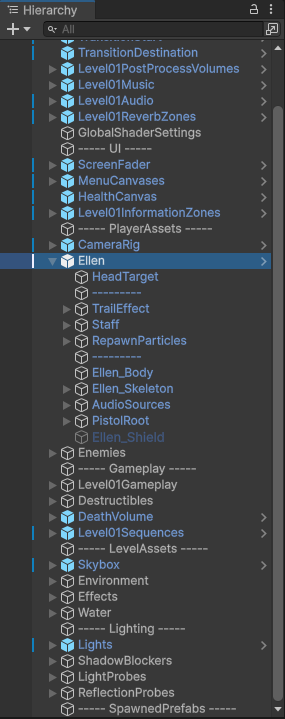
\includegraphics[width=0.9\textwidth]{content/Research/Unity-Hierarchy.png}
        \caption{Screenshot of the Unity engine's Hierarchy view, showing a tree of all the Game Objects present in the scene.}
        \label{fig:unity-hierarchy}
    \end{minipage}
    \hfill
    \begin{minipage}[c]{0.5\linewidth}
        \includegraphics[width=\textwidth]{content/Research/Unity-Inspector.png}
        \caption{Screenshot of the Unity engine's Inspector view, showing the properties and components of a selected Game Object.}
        \label{fig:unity-inspector}
    \end{minipage}%
\end{figure}


\begin{figure}[h]
    \begin{minipage}[c]{0.5\linewidth}
        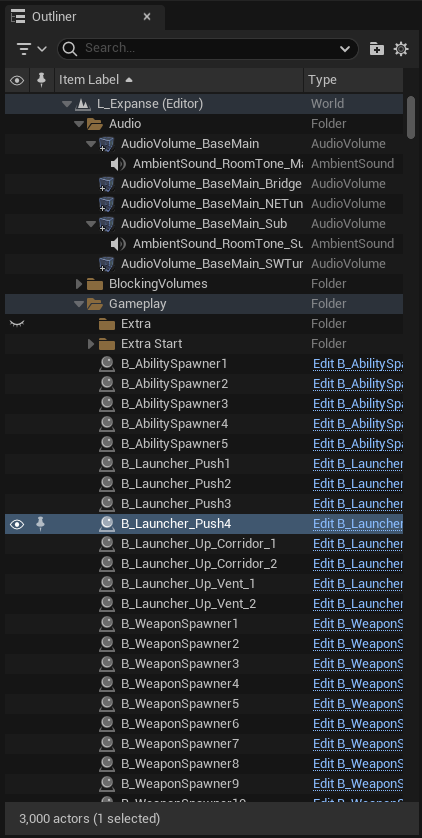
\includegraphics[width=0.9\textwidth]{content/Research/UE5-Outliner}
        \caption{Screenshot of the Unreal Engine's Outliner view, showing a tree of all the Actors present in the scene}
        \label{fig:ue5-outliner}
    \end{minipage}
    \hfill
    \begin{minipage}[c]{0.5\linewidth}
        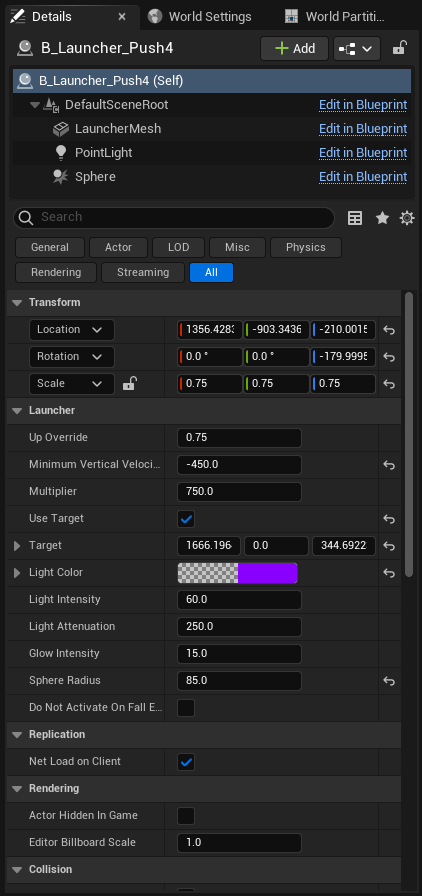
\includegraphics[width=\textwidth]{content/Research/UE5-Details}
        \caption{Screenshot of the Unreal Engine's Details view, showing the properties and components of a selected Actor.}
        \label{fig:ue5-details}
    \end{minipage}%
\end{figure}


\begin{figure}
    \includegraphics[width=1\textwidth]{content/architecture/startup.eps}
    \caption{Sequence diagram of the start-up of the engine}
    \label{fig:startup-diagram}
\end{figure}

\begin{figure}
    \includegraphics[width=1\textwidth]{content/architecture/startup-init.eps}
    \caption{Detailed sequence diagram of module initialization}
    \label{fig:startup-init-diagram}
\end{figure}

    \newpage
    \chapter*{Document info}
    This document was compiled from the Umbra monorepo on \today \\
    Commit: \gitcommit \\
    Branch: \gitbranch \\

    %\label{page:last}
\end{document}
